%-*- program: pdflatex -*-
%-*- program: bibtex -*-
%-*- program: pdflatex -*-
%-*- program: pdflatex -*-


% --------------------------------------------------------------
% Preamble
% --------------------------------------------------------------

\documentclass[english,natbib,man,floatsintext]{apa6}
% \usepackage{arxiv}
\usepackage[english]{babel}
\usepackage[utf8]{inputenc} % allow utf-8 input
\usepackage[T1]{fontenc}    % use 8-bit T1 fonts
\usepackage{url}            % simple URL typesetting
\usepackage{hyperref}       % hyperlinks
\usepackage{xcolor}
\hypersetup{
    colorlinks,
    linkcolor={red!50!black},
    citecolor={blue!50!black},
    urlcolor={blue!80!black}
}
\usepackage{booktabs}       % professional-quality tables
\usepackage{tabularx}
\usepackage{amsfonts}       % blackboard math symbols
\usepackage{nicefrac}       % compact symbols for 1/2, etc.
\usepackage{microtype}      % microtypography
\usepackage{gensymb}        % degree, angle symbols

% for math equations and symbols
\usepackage{amsmath} 
\usepackage{amssymb} 
\newcommand{\E}{\mathbb{E}}
\newcommand{\SD}{\mathit{SD}}
\newcommand{\SE}{\mathit{SE}}
\newcommand{\BF}{\mathit{BF}}
\DeclareMathOperator\arctanh{arctanh}

% This prevents placing floats before a section.
\usepackage{placeins}

% bibliography
% \usepackage{natbib}

% allows for floats when doing jou or doc style
\usepackage{graphicx}      
\graphicspath{{./figs/}}  

% linenumbers
\usepackage[mathlines]{lineno}

% in APA man mode captions are too large
% making sure they are reasonable
\usepackage{setspace}
% \usepackage[font=singlespacing]{caption}
% \captionsetup{font=singlespacing}

%%% some support for commenting

\usepackage{color}
\definecolor{Blue}{RGB}{0,0,255}
\definecolor{Red}{RGB}{255,0,0}
\newcommand{\jo}[1]{\textcolor{Red}{[Jacob: #1]}}  
\newcommand{\hs}[1]{\textcolor{Blue}{[Hrvoje: #1]}} 
% \newcommand{\jo}[1]{}  
% \newcommand{\hs}[1]{} 


% ---------------------------------------------------------
% Title, authors
% ---------------------------------------------------------

\title{The visual environment, attention and decision making}

% Alternatives
% A meta-analysis of eye movements in decision making
% The visual environment influences attention during decision making
% The visual environment, attention and decision making
% A meta analysis of influence of the visual environement factors on  attention in decision making

%%% arxiv style

% \author{
%   Jacob L. Orquin\thanks{Correspondence concerning this article should be addressed to Jacob L. Orquin, Department of Management/MAPP, Aarhus University, Fuglesangs alle 4, 8210 Aarhus V - Denmark. E-mail: jalo@mgmt.au.dk. Data and scripts are available at: \url{https://osf.io/buk7p/}. This research was supported by the Independent Research Fund Denmark, grant number: 8046-00014A. The authors thank Martin Meissner, Tobias Otterbring, Sonja Perkovic, and Valdimar Sigurdsson for feedback on earlier versions of the manuscript.}, Erik S. Lahm, Hrvoje Stojić
% }

%%% APA style

\shorttitle{The visual environment, attention and decision making}

\threeauthors{Jacob L. Orquin*}{Erik S. Lahm}{Hrvoje Stojić}
\threeaffiliations{Aarhus University and Reykjavik University}{Aarhus University}{University College London}

\authornote{Jacob L. Orquin and Erik S. Lahm, Department of Management/MAPP, Aarhus University, Fuglesangs alle 4, 8210 Aarhus V - Denmark; Hrvoje Stojić, Max Planck UCL Centre for Computational Psychiatry and Ageing Research, University College London, 10-12 Russell Square, London, WC1B 5EH, United Kingdom. The authors thank Martin Meissner, Tobias Otterbring, Sonja Perković, and Valdimar Sigurdsson. This research was supported by the Independent Research Fund Denmark, grant number: 8046-00014A. *Correspondence concerning this article should be addressed to Jacob L. Orquin, Department of Management/MAPP, Aarhus University, Fuglesangs alle 4, 8210 Aarhus V - Denmark. E-mail: jalo@mgmt.au.dk. 
}

\rightheader{Orquin, Lahm, Stojic}
\leftheader{The visual environment, attention and decision making}


% \begin{document}
% \maketitle

% ---------------------------------------------------------
% Abstract
% ---------------------------------------------------------


\abstract{% NHB limit: 150 words
Visual attention is fundamental to most everyday decisions, and governments and companies spend vast resources on competing for it. In natural choice environments options differ on a variety of visual factors, such as salience, position or surface size. However, most decision theories ignore such visual factors, focusing on cognitive factors such as preferences as determinants of attention. To provide a systematic review of how the visual environment guides attention we meta-analyze studies on eye movements in decision making. Results show that cognitive factors indeed matter the most to attention. However, visual factors like surface size, positioning, and set size also have sizable effects on attention, independently of cognitive factors. While much research is concentrated on salience, we show that it has little or no effect on attention. Understanding real world decision making will require integration of both cognitive and visual factors in future theories of attention and decision making.
}

\keywords{eye movements, decision making, meta-analysis, top-down control, bottom-up control} 


\begin{document}
% \raggedbottom
\linenumbers
\maketitle

% -------------------------------------------------------
% Introduction
% -------------------------------------------------------

\section{Introduction}

% \section{Motivation and Problem}

Decision making often takes place in environments where relevant information needs to be acquired visually. In such visual environments choice alternatives can differ in their position, surface size, salience and many other visual properties. Consider encountering a product with a surprising color on a supermarket shelf, or a restaurant menu where certain items take a prominent position and perhaps have an accompanying picture. Such visual properties have been shown to influence our attention \citep{corbetta2002a,borji2012a, dehaene2003a,clarke2014a,rosenholtz2007a}. There is growing evidence showing that attention plays an important role in decision making \citep{gidloef2017a,krajbich2010a,stojic2020uncertainty, callaway2019a,gluth2018, gluth2020}, and can even causally affect choices \citep{ghaffari2018a, paernamets2015a, shimojo2003a}. However, the role of visual environment factors is almost completely absent from prominent decision theories. In most theories, cognitive factors such as goals in the decision task determine the relevance of objects and, either explicitly or implicitly, whether and when we look at them. Here, we ask whether decision research is building on correct assumptions about visual attention and the role of the visual environment, and provide an empirical assay of the relative importance of various visual and cognitive factors to guide further theory development.\\

% \section{Decision research (mostly) ignores bottom-up factors}
Most decision research considers attention to be determined by the decision process, that it is driven by the goal relevance of objects rather than the visual properties of these objects. In many prominent decision making models this assumption is implicit. Consider, for example, the prospect theory model of how probabilities and values of choice alternatives are integrated to arrive at a preferential choice \citep{tversky1979}. Alternatives are treated equally according to this model, and nothing in the model indicates that one piece of information would attract more attention than the other. Prospect theory and other related variants of expected utility theory are focused on capturing the final choices, not the process of how people arrive at choices. However, popular process-oriented decision making models commit to similar assumptions about attention. Consider, for example, satisficing, elimination-by-aspect, or the lexicographic heuristics \citep{payne1988, simon1956a}. While these models all specify different information search processes, they make similar implicit assumptions about the nature of visual search and hence attention in decision making. These  models assume that the information search is determined by a search rule inherent to the decision process, e.g. attend to alternatives one at a time until a satisfactory alternative is found \citep{stuttgen2012}, or attend to information cues in order of their predefined validity until a cue is found that identifies the best alternative \citep{krefeld-schwalb2019a}.\\ 

In recent sequential sampling models of decision making attention has had a more explicit role. Sequential sampling models assume that stochastic evidence for an alternative is accumulated over time and when the integrated evidence reaches a threshold a choice is made. This is a process-oriented model that aims to capture how people balance the value of accumulating more information with the cost of taking more time to reach a decision \citep{forstmann2016}. In two influential variants of these models attention plays an important role, by determining how evidence is sampled in favor of choice alternatives \citep{busemeyer1992} or by determining the weight assigned to the evidence \citep{krajbich2010a, thomas2019}. In these models, attention fluctuates randomly between choice alternatives or choice attributes until a choice is made. The implicit assumption being, that in the long run attention is uniformly distributed over alternatives and attributes. This is a stochastic equivalent to a maximizing decision rule such as the weighted additive which assumes that a decision maker attends equally to all information \cite{gloeckner2011a, payne1988}. In other words, even though attention exerts an influence on choice, this influence is random and neither controlled by goals nor the visual environment. Recently, sequential sampling models have been proposed in which attention is guided by the value of choice alternatives \citep{callaway2019a, gluth2018, gluth2020}. This assumption is supported by empirical findings demonstrating value based attentional capture, i.e. the effect that objects associated with rewards capture attention \citep{lepelley2015}. The models are reminiscent of an earlier idea by \cite{shimojo2003a} who proposed that decision makers attend preferentially to high value alternatives, which increases their value further, thus creating a feedback loop and increasing likelihood of gazing at the ultimately chosen alternative.\\ 

There are a few studies that proposed decision making models where attention is not driven only by the goal relevance of alternatives, but also by their visual properties, focusing on salience, i.e. the visual conspicuousness of a stimulus relative to its surroundings. For example, \cite{towal2013a} showed that salience continuously influences the decision process by making some choice alternatives more likely to attract fixations, but it does not influence the drift rate, i.e. the speed of accumulating evidence, towards salient choice alternatives directly. \cite{chen2013} provided evidence that salience can determine the onset of drift towards a choice alternative, but not the drift rate itself. Finally, \cite{navalpakkam2010} showed that decision makers in a reward harvesting task made choices by combining value and salience, consistent with an ideal Bayesian observer. This work suggests that salience can influence the decision process directly rather than by biasing attention.\\ 

% \section{Why do we need bottom up factors in decision making models?}

The assumption in decision science about cognitive factors being the only or main factor driving attention in decision making is inconsistent with a number of findings. \cite{vanderlans2008}, for instance, find that 2/3 of variance in attention is due to factors in the visual environment, unrelated to the decision task, and \cite{towal2013a} find that 1/3 of variance is due to stimulus factors. There are also several model free studies showing comparative effects of cognitive and visual factors on attention in decision making \citep{gidloef2017a, orquin2015a, orquin2019a}. Moreover, there is evidence that the visual environment influences choices by biasing visual attention. For instance, decision irrelevant visual factors have been shown to influence choices by changing the amount of gaze \citep{peschel2019, chandon2009a} or the order of gaze \citep{reeck2017a}. Even studies examining purely cognitive models of decision making often implicitly acknowledge the influence of visual factors by taking great effort to eliminate them by controlling the size, position, and salience of information \citep{brandstatter2014, gloeckner2011a, perkovic2018}.\\

Further evidence for the role of visual factors comes from vision science research. The few studies that modelled the influence of the visual environment on attention in decision making focused exclusively on salience \citep{chen2013,navalpakkam2010, towal2013a}. This focus seems justified - a great deal of research in vision science has concentrated on salience, for a review see \cite{borji2012a}. The term salience refers to stimuli that differ from their surroundings in terms of visual conspicuity and it has been shown that observers are more likely to gaze at stimuli that are high in salience \cite{itti2000}. However, there has been much debate about the role of salience in guiding attention some arguing that it plays no role in, for instance, real world behavior \citep{tatler2011a}. Besides salience, there are at least three other visual factors that are likely to guide attention in decision making \citep{orquin2013a, wedel2008}.\\

One factor is the relative surface size of stimuli, which refers to the proportion of the visual environment occupied by the stimulus \citep[for a review see][]{peschel2013a}. Increasing the surface size of choice alternatives has been shown to increase gaze by up to 25 \% \citep{chandon2009a}. Increments to surface size exhibit a diminishing marginal effect on eye movements \citep{lohse1997a}. A second factor is the position of stimuli which has been shown to influence eye movements and is sometimes corrected for in vision research models when estimating the influence of other variables of interest \citep{clarke2014a}. In a decision context alternatives are normally placed in different spatial locations, which means that position effects like left-to-right (reading) direction and centrality are likely to influence eye movements and choices \citep{atalay2012a, meissner2016a}. A third factor is the set size which in a decision context normally is operationalized as the number of alternatives or attributes. Increasing the set size generally slows reaction times to identify search targets \citep{wolfe2010} and may also increase the visual complexity by the addition of more and different visual stimuli. Visual complexity has been shown to increase the difficulty and amount of visual search \citep{rosenholtz2007a}. An important point about these visual factors is that all four are likely to vary in natural environments and have been shown to affect attention simultaneously \citep{orquin2019a}. While decision research often sees the visual environment as a nuisance factor and try to eliminate its influence on decision making \citep{brandstatter2014, gloeckner2011a, perkovic2018}, companies and governments often use the same factors to compete for the attention of consumers and citizens \citep{pieters2017, orquinwedel2020}.\\   

Despite these findings on the presumed importance of visual factors in attention and decision making, they have had only a small impact on theory development. While attention and cognitive influences recently started playing a prominent role in decision theories \citep{callaway2019a, gluth2018, gluth2020, krajbich2010a, noguchi2018, thomas2019, usher2019}, the role of visual factors has been largely ignored. There are only a few studies that have proposed and tested models that incorporate the influence of the visual environment on attention in decision making \citep{chen2013, navalpakkam2010, towal2013a}. Moreover, these studies have focused exclusively on salience, despite the other visual factors that are likely to be relevant as well and their joint contribution. A systematic review that provides evidence on how important visual factors are individually, as well as relative to cognitive factors, would give a new impetus to research and theory development incorporating the role of the visual environment; or justify the lack of it. The increasing availability of eye-tracking equipment has paved the way for such a review. Eye-tracking provides a way to unobtrusively measure the influence of both visual and cognitive factors on attention in decision tasks. In the last two decades numerous model free eye-tracking studies appeared, situated in a decision context. These studies span many disciplines, from behavioural economics and consumer psychology to cognitive psychology, computational neuroscience and vision science, which potentially explains why such a review has not been done before.\\

% \section{Study approach} 

Here, we assess the importance of the visual environment in decision making by empirically examining the magnitude of effects of various visual factors on attention in decision making and comparing them with cognitive factors. We focus on four visual factors -- salience, position, surface size and set size -- and three cognitive factors -- task effects, preferential viewing and choice bias. We collect effect sizes from studies on eye movements in decision making and meta-analyze them to get reliable effect estimates. To do so, we developed new methods to address methodological challenges of meta-analysing eye movement data. Our findings show that among the visual factors position in the centre of the field of view has the largest effect, while salience has the smallest effect on attention. Relative to cognitive factors, visual factors have somewhat smaller effects on eye movements.  However, since all visual factors can influence attention simultaneously, in cases with multiple factors \citep{gidloef2017a, orquin2019a}, these could jointly have a larger influence than cognitive factors. Overall, these results show that characteristics of the visual environment have reliable effects on eye movements in decision making and that the effects are present across various decision contexts and tasks. This suggests that future theories and models of decision making should integrate visual factors directly rather than see them as nuisance factors.


% -------------------------------------------------------
% Results
% -------------------------------------------------------

\section{Results}

Our initial literature search retrieved 1981 articles, of which 454 remained after screening of the title and abstract. Following a more detailed evaluation of whether studies were on decision making and used eye-tracking, we identified 291 articles as potentially eligible studies. Based on detailed inspection of their full texts, 58 articles satisfied all inclusion criteria and were included in the meta-analysis. Figure~\ref{fig:flow_diagram} illustrates the PRISMA flow diagram \citep{moher2009preferred}. Many of the articles consisted of multiple experiments and some experiments operationalized more than one factor. This resulted in 106 independent effect size estimates, out of which 39 were effects of visual factors and 67 were effects of cognitive factors.


\begin{figure}[H]
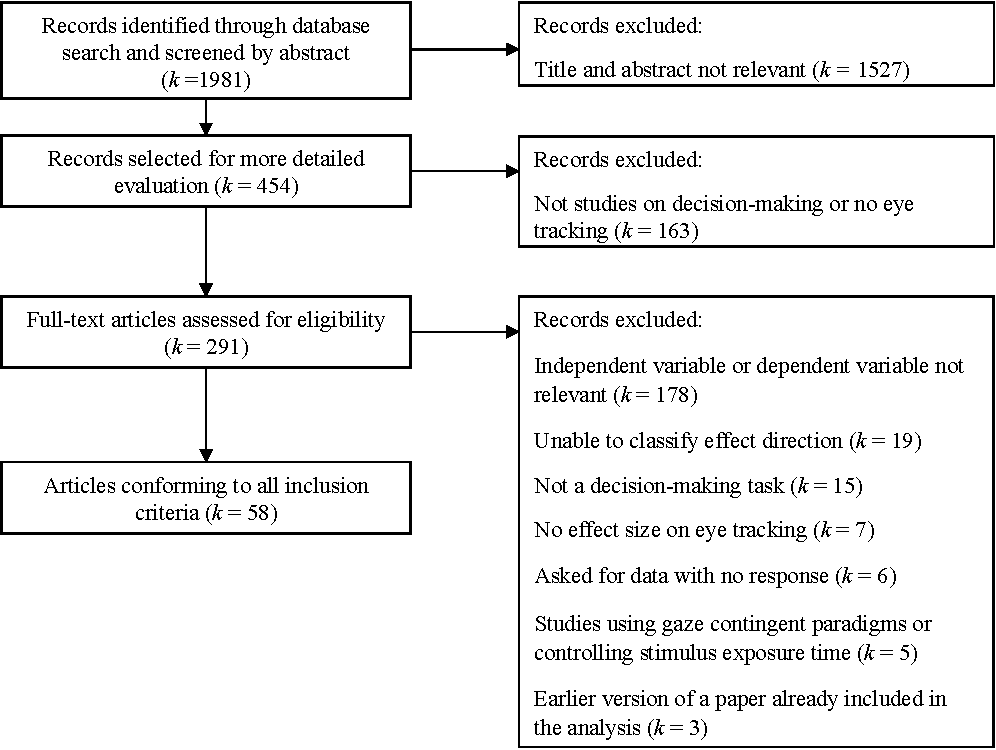
\includegraphics[width=0.8\textwidth]{prisma}
\centering
\caption{The PRISMA flow diagram showing the results of the literature search.}
\label{fig:flow_diagram}
\end{figure}


Meta-analyses of eye movements are relatively rare and it could be due to some methodological challenges in combining effect sizes from different eye-tracking studies. Two main challenges are how to handle measurement validity across eye-tracker types and how to compare different eye movement dependent variables. To handle these issues, we developed correction procedures to be integrated in a psychometric meta-analysis \citep{hunter2004a}, which allows us to quantify the interference of measurement validity or multiple metrics. The measurement validity issue stems from differences in the accuracy and precision of eye-tracking equipment \citep{holmqvist2015a}, which can affect the data quality and bias effect sizes \citep{orquin2016a}. We developed a correction method that relies on an empirical estimate of the relationship between eye-tracker characteristics and observed effect sizes (see \textit{Methods}; Figure~\ref{fig:ET_accuracy_effectsize}; Table~\ref{tab:eyetracker_specifications}) since there are multiple eye movement dependent variables commonly used. Most metrics are based on fixations -- defined as maintaining the gaze on a single location or area of interest (AOI), such as fixation count, fixation likelihood, total fixation duration and so on. This leads to a potential issue with comparing effect sizes reported with different dependent variables. We developed a correction method that makes the dependent variables comparable, where we empirically estimate correction factors based on a subset of studies in our sample that report multiple dependent variables (see \textit{Methods}; Figure~\ref{fig:metric_correction}; Table~\ref{tab:metric_correction}). This method allowed us to transform all effect sizes to a single metric; we decided for fixation count which was used in all meta-analyses. 

In what follows, we first analyse the group of visual factors and then the group of cognitive factors. We perform meta-analysis on each individual factor  separately. We next perform a small moderator analysis and finish with an analysis of publication bias in all the meta-analyses.  


\subsection{Visual factors}

We focused on four major groups of visual factors -- salience, position, surface size and set size (see \textit{Methods} for coding procedure). The summary effects of the visual factors on attention during decision making show that, except for salience and left vs right position, all factors have medium effect sizes ranging from $\rho = 0.29$ to $\rho = 0.43$, with moderate amounts of heterogeneity ranging from $I^2 = 46.3\%$ to $I^2 = 55.8\%$ (Table~\ref{tab:main_results} and Figure~\ref{fig:forest_plots_visual}). Salience, which so far has been taking the central stage in vision science, surprisingly has the smallest summary effect ($\rho = .11$; 95\% confidence interval (CI) = $[-0.02,0.24]$; $p=0.098$), practically indistinguishable from a null effect. When we adjust the summary effect using the trim and fill method (see \textit{Publication bias} section), one imputed study decreases the effect size to $\rho = 0.10$ (95\% CI = $[-0.02,0.23]$; Table~\ref{tab:main_results}). The position factor was decomposed into a left-vs-right (reading direction) and a center factor (tendency to attend to the center of the visual field). The center factor has the largest summary effect among visual factors ($\rho = .43$; 95\% CI = $[0.27,0.60]$; $p<0.001$), which decreases somewhat after the trim and fill adjustment ($\rho = .39$; 95\% CI = $[0.22,0.56]$; $p<0.001$; Table~\ref{tab:main_results}). 

Overall, three factors show reliable effect sizes: center position, surface size and set size. Considering that there is no (natural) environment free of visual factors, it is reasonable to expect that multiple visual factors influence eye movements at the same time. Hence, even though individual effect sizes are not large, jointly they can be a major driver of attention during decision making.


% \caption{Main results of the meta-analysis divided into independent variable subgroups }
% \label{tab:main_results}
% latex table generated in R 3.6.3 by xtable 1.8-4 package
% Sat Jun 20 12:32:29 2020
\begin{table}[ht]
\centering
\caption{Main results of the meta-analysis, divided into visual and cognitive factor groups, and individual factors within them. The most important values are the corrected effect size estimate, $\rho$, and the associated heterogeneity, $I^2$. Results of trim and fill analysis are in the parentesis.} 
\label{tab:main_results}
\begingroup\small
\begin{tabular}{lp{0.03\linewidth}p{0.05\linewidth}p{0.07\linewidth}p{0.07\linewidth}p{0.07\linewidth}p{0.07\linewidth}p{0.07\linewidth}p{0.07\linewidth}p{0.07\linewidth}}
  \hline
Group & $k$ & $N$ & $\rho$ & SE & $Z$ & $p$ & $\textrm{CI}_{95}$ LL & $\textrm{CI}_{95}$ UL & $I^2$ \\ 
  \hline
\textbf{Visual factors} &  &  &  &  &  &  &  &  &  \\ 
  Salience & 9 (1) & 530 & 0.11 (0.11) & 0.066 (0.121) & 1.659 (0.911) & 0.097 (0.362) & -0.02 (-0.127) & 0.24 (0.335) & 0 \\ 
  Surface size & 6 (0) & 740 & 0.396 (0.508) & 0.108 (0.188) & 3.682 (2.986) & 0 (0.003) & 0.185 (0.19) & 0.607 (0.73) & 55.31 \\ 
  Left vs right position & 3 (0) & 415 & 0.316 (0.485) & 0.213 (0.32) & 1.484 (1.652) & 0.138 (0.099) & -0.101 (-0.098) & 0.733 (0.82) & 46.04 \\ 
  Center position & 11 (0) & 912 & 0.434 (0.622) & 0.086 (0.209) & 5.065 (3.48) & 0 (0.001) & 0.266 (0.308) & 0.602 (0.814) & 49.92 \\ 
  Set size & 10 (0) & 610 & 0.29 (0.348) & 0.094 (0.126) & 3.095 (2.891) & 0.002 (0.004) & 0.106 (0.116) & 0.473 (0.544) & 55.06 \\ 
  \textbf{Cognitive factors} &  &  &  &  &  &  &  &  &  \\ 
  Task instructions & 26 (0) & 1990 & 0.419 (0.516) & 0.059 (0.084) & 7.146 (6.789) & 0 (0) & 0.304 (0.385) & 0.534 (0.626) & 43.75 \\ 
  Preferential viewing & 21 (0) & 2014 & 0.476 (0.75) & 0.086 (0.171) & 5.544 (5.677) & 0 (0) & 0.308 (0.563) & 0.645 (0.864) & 79.87 \\ 
  Choice bias & 18 (6) & 625 & 0.695 (0.949) & 0.086 (0.263) & 8.088 (6.929) & 0 (0) & 0.527 (0.863) & 0.864 (0.981) & 67.51 \\ 
   \hline 
 \multicolumn{10}{p{0.9\textwidth}}{\scriptsize{\textit{Note.} $k$ = number of studies (for trim and fill analysis number of imputed studies); $N$ = number of participants; $\rho$ = unattenuated effect size estimate, SE = standard error of estimate; $Z$ = Z statistic; $p$ = significance level; $\textrm{CI}_{95}$ LL = lower limit of the 95\% confidence interval; $\textrm{CI}_{95}$ UL = upper limit of the 95\% confidence interval, $I^2$ = within-group heterogeneity.}} 
\end{tabular}
\endgroup
\end{table}



\begin{figure}[!H]
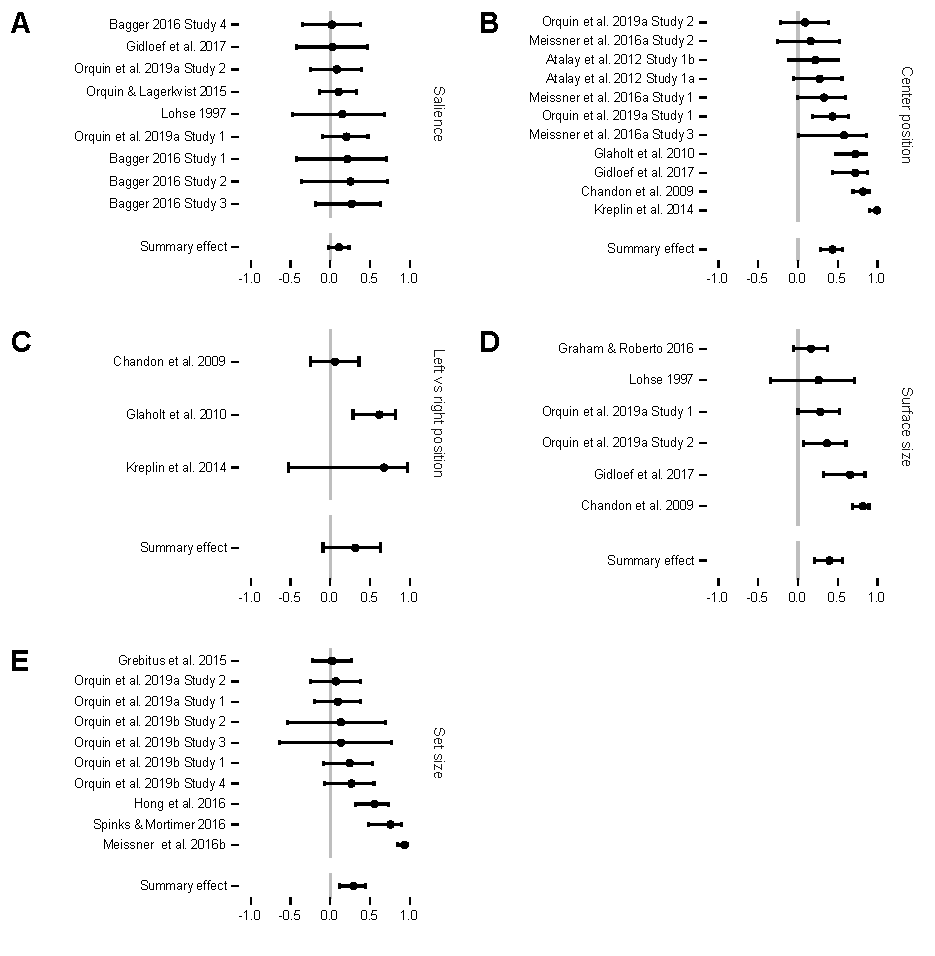
\includegraphics{forest_plots_visual}
\centering
\caption{Effect sizes of the visual factors are moderate, except for salience and left-vs-right position, which have small effect sizes, if any. Forest plots show the unattenuated effect size correlations for each study in a group, as well as average effect across the group. Forest plot in (A) shows the effect sizes for salience factor, in (B) for center position, in (C) for left vs right position, in  (D) for surface size, and in (E) for set size factor. Error bars represent the 95\% confidence interval around the mean.}
\label{fig:forest_plots_visual}
\end{figure}


\subsection{Cognitive factors}

Previous research has identified a wide range of cognitive factors that influence attention, such as goals, task instructions, and preferences \citep[for a review see][]{orquin2013a}. Here, we divided cognitive control factors into three groups: task instruction, preferential viewing and choice bias. 

In studies on task instructions, participants receive instructions concerning a specific decision goal, and with that, what is relevant to gaze at. For instance, the participants may be instructed on the validity of stimulus attributes \citep{krefeld-schwalb2019a}, or infer the level of validity themselves \citep{bialkova2014a}. In preferential viewing studies, the relevance should be equal to the subjective preferences. For example, some alternatives have higher subjective values than others \citep{kim2012a}. Because of this qualitative difference between the two domains, we treated studies on task instructions and preferential viewing separately. The inspection of the effect sizes reveals that the summary effects in the two types of studies are moderate and similar in magnitude -- in task instructions $\rho = .42$ (95\% CI = $[0.30,0.53]$; $p<0.001$) and in preferential viewing $\rho = .48$ (95\% CI = $[0.31,0.64]$; $p<0.001$; Table~\ref{tab:main_results} and Figure~\ref{fig:forest_plots_cognitive}). Using a Wald test, we find that effect sizes of task instructions and preferential viewing are unlikely to differ, $z=-0.033$, $p=0.399$. When we adjust the effects for publication bias using the trim and fill method, the effect size for task instructions decreases to $\rho = 0.38$ (95\% CI = $[0.26,0.51]$; Table~\ref{tab:main_results}) and for preferential viewing to $\rho = 0.37$ (95\% CI = $[0.19,0.55]$; Table~\ref{tab:main_results}). This result suggests that it makes no difference to eye movements whether the relevance of information is defined according to an externally specified goal or according to preferences. 

Choice bias refers to an effect in attention whereby decision makers spend more time gazing at the eventually chosen alternative. This effect, originally introduced by Shimojo and colleagues \citep{shimojo2003a} as a ``gaze-cascade'' effect, is well-established in the literature, prompting us to study it as a separate factor. This factor consists of studies reporting the difference in eye movements between the chosen alternative and all other (not chosen) alternatives. We find that choice bias has a large effect on eye movements, $\rho = 0.69$ (95\% CI = $[0.53,0.86]$; $p<0.001$) (Table~\ref{tab:main_results} and Figure~\ref{fig:forest_plots_cognitive}). The effect decreases to moderate size after publication bias adjustment ($\rho = 0.49$; 95\% CI = $[0.31,0.67]$; Table~\ref{tab:main_results} in parenthesis)


\begin{figure}[!H]
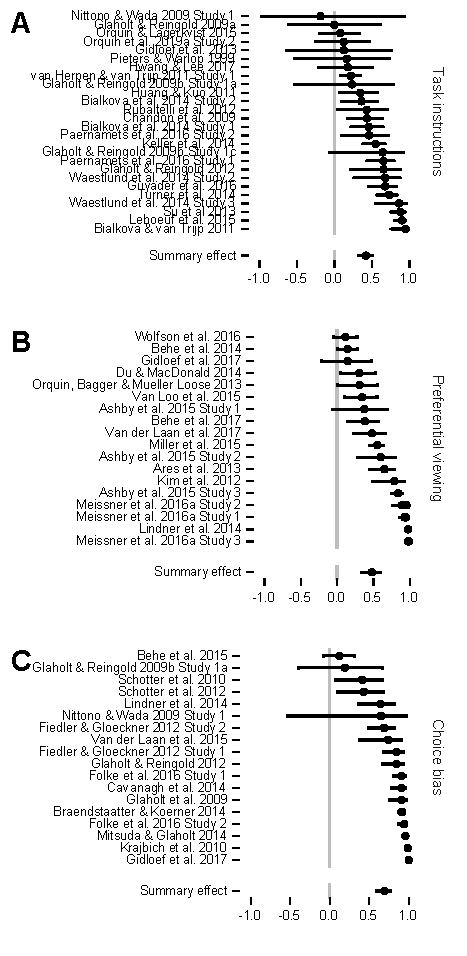
\includegraphics{forest_plots_cognitive}
\centering
\caption{Effect sizes of the three cognitive factors are moderate to large. Forest plots show the unattenuated effect size correlations for each study in a group, as well as average effect across the group. Forest plot in (A) shows the effect sizes for task instructions factor, in (B) for preferential viewing, and in (C) for the choice bias factor. Error bars represent the 95\% confidence interval around the mean.}
\label{fig:forest_plots_cognitive}
\end{figure}


\subsection{Moderator analyses}

Alternatives that participants in judgment and decision making studies choose between can often be decomposed into constituent elements, commonly called attributes, cues or features \citep{payne1988,tversky1972elimination,stojic2020s,gigerenzer1996reasoning,schulz2018putting,hogarth2007heuristic}. For example, in classical lottery tasks \citep{tversky1979}, the probabilities and values of an alternative can be viewed as attributes. Or, in multi-cue judgment tasks, alternatives are more explicitly composed of cues -- university, major football team or main city in the German city size task \citep{gigerenzer1996reasoning}. This has consequences for both modelling of decision processes and units of analysis. Consequently, some studies in our sample focused on attention effects at either alternative or attribute level, or both. This was in particular the case for studies involving set size, task instructions, and preferential viewing factors. Since the alternative vs attribute dimension might be an important moderator in these groups, we decomposed them further with regards to the effect of alternatives vs attributes (Table~\ref{tab:mod_results} and Figure~\ref{fig:forest_plots_altatt}). Moderator analyses shows a support for the alternative vs attribute moderator across set size, $Q_M(1)=4.765$, $p=0.029$, weak support for preferential viewing, $Q_M(1)=4.312$, $p=0.038$, and no support for task instructions, $t=-0.213$, $p=0.835$. It is noteworthy that effect sizes are consistently larger when operationalized at the level of alternatives compared to attributes (Table~\ref{tab:mod_results} and Figure~\ref{fig:forest_plots_altatt}). 

We also performed a moderator analysis for the choice bias factor, to assess whether the effect is driven by preferential viewing as proposed by \cite{shimojo2003a}. We compare studies with preferential vs inferential choice tasks and find no support for moderation by decision type, $Q_M(1)=0.057$, $p=0.811$, and only report results for the main group. 

\subsection{Publication bias}

We assessed potential publication bias using trim and fill analysis of each factor \citep{duval2000trim}. In addition, we plotted the  Fisher transformed correlation coefficients of each study by its respective standard error (so-called funnel plots; Figure~\ref{fig:funnel_plots} for main results, and Figure~\ref{fig:funnel_plots_altatt} for moderator analyses). The symmetry of the funnel plots provides a qualitative picture of whether there is a file drawer problem. We expect that studies with smaller sample sizes and hence higher standard errors yield more variable effect sizes, the smallest of which are less likely to be published, leading to an asymmetric funnel plot. Judging from the funnel plots, it is not obvious whether there is a problem with publication bias. However, the trim and fill analysis resulted in a downward adjustment of the average effect size for most of the factors. The corrected effect sizes in Table~\ref{tab:main_results} (in parentheses) provide a more conservative estimate of the true population effects, but are also subject to some uncertainty. Specifically, the interpretation of the corrected results may be biased due to heterogeneity in many of the factors as well as a relatively small number of studies in the group of visual factors. 


\begin{figure}[!H]
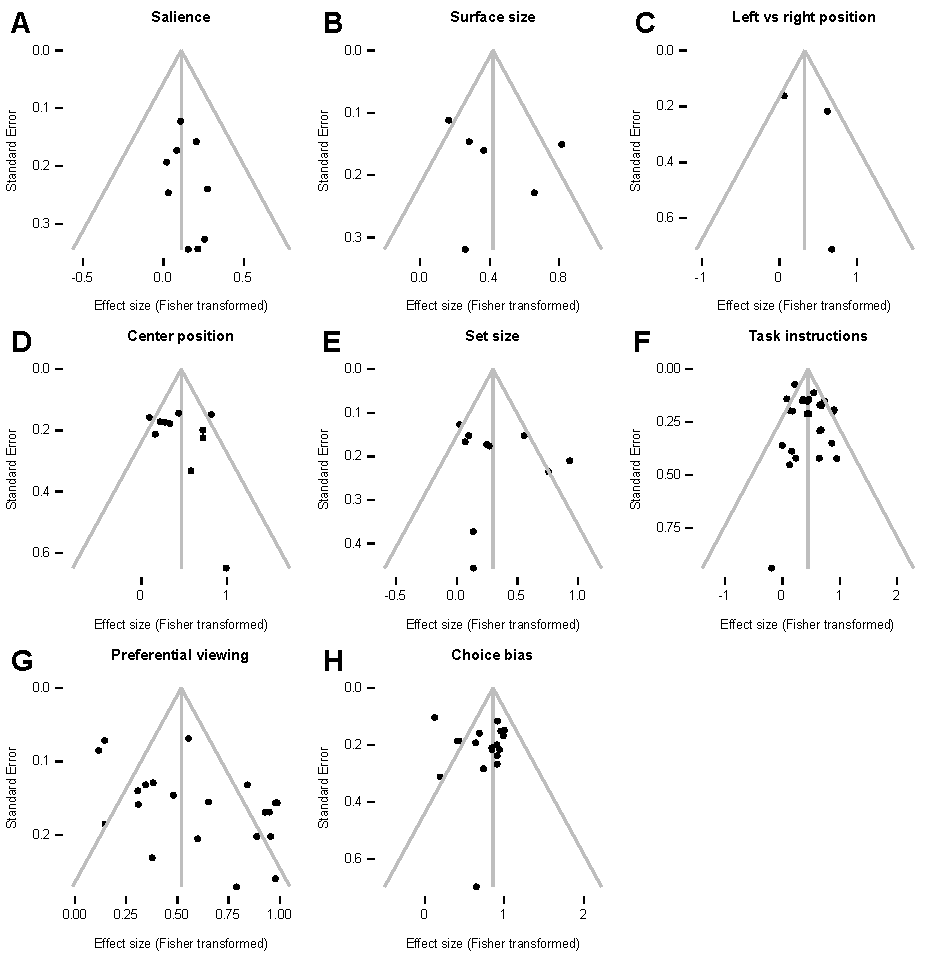
\includegraphics{funnel_plots}
\centering
\caption{Funnel plots for each factor that can be used as a qualitative check of a publication bias. Points are Fisher transformed correlation coefficients against their standard error. Asymmetric distributions of points can indicate the presence of publication bias since smaller studies (those with higher standard errors) have more variable effect sizes and are less likely to be published unless the effect is large. Funnel plot for (A) salience, (B) surface size, (C) left vs right position, (D) central position, (E) set size, (F) task instructions, (G) preferential viewing, and (H) choice bias.}
\label{fig:funnel_plots}
\end{figure}


% -------------------------------------------------------
% Discussion
% -------------------------------------------------------


\section{Discussion}

%%% 1. Brief reminder what the study is about
For the better part of our daily lives, we attend to and gather information using our eyes and consequently many of the decisions we make, small or large, depend on visual attention. In this article, we attempt to answer to what extent the visual environment guides our attention during decision making. To this end, we meta-analyze empirical studies on eye movements in decision making. We distinguish between visual environment factors such as salience, surface size, set size, and position, and compare them to cognitive factors such as preferential viewing, task instructions and choice bias. We identify 106 effect sizes across 58 studies and perform a psychometric meta-analysis to control for methodological issues that arise when meta-analysing eye-movement studies.\\ 

% main findings - importance of visual factors 
% att odds with vast majority of current theories
Except for salience and left vs right position, the results show that visual factors have medium effect sizes. In comparison, effect sizes of the three cognitive factors are slightly larger, choice bias in particular. In laboratory environments, it is possible, and often desirable, to control for visual factors, but in natural environments where no such control or counterbalancing takes place, all visual factors could influence eye movements simultaneously \citep{orquin2019a}. Furthermore, there are potentially other less researched visual factors not covered in our study that influence eye movements, e.g. motion or sudden onsets are known to capture eye movements involuntarily \citep{abrams2003, jonides1988}, but have not been studied in decision making. Thus, visual factors might be major drivers of attention in real world decision making, well aligned with previous suggestions that 2/3 of variance in eye movements is due to visual factors \cite{vanderlans2008}. These findings are clearly at odds with most decision making models that assume equal attention to all stimuli \citep{tversky1979,payne1988, simon1956a}, but also with models that assume no role of cognitive factors in guiding attention in decision making \citep{busemeyer1992, krajbich2010a} or no role of visual factors in guiding attention \citep{callaway2019a, gloeckner2011a, gluth2018, gluth2020}.\\ 

% integrating visual and cognitive factors in models of attention and
% decision making
Our findings will hopefully reinvigorate the line of research integrating visual and cognitive factors in driving attention in decision making. Important first steps have been taken by \cite{chen2013}, \cite{navalpakkam2010}, and \cite{towal2013a}, who developed models integrating the role of salience in decision making. Their sequential sampling based models suggest that salience may influence the onset of drift or perhaps the amount of drift. This research left us with some important questions unanswered and new research should tackle these first. For example, we still do not know whether salience consistently biases attention in decision situations, or if the effect is limited to decisions under time pressure as in \citep{chen2013, navalpakkam2010, towal2013a, milosavljevic2012a}? If salience mainly influences attention immediately after stimulus onset \citep{theeuwes2010, orquin2015a}, the effect of salience on attention and choice may diminish as the decision time extends or it may have no bearing on the effect if salience influences the onset of drift as suggested by \cite{chen2013}. While there are still many unanswered questions about the mechanisms underlying the interactions between salience and decision processes, hardly any have been addressed concerning the other visual factors. Our findings are silent on the mechanisms and a pressing next step is to integrate multiple visual factors in decision making models to improve our understanding how exactly they jointly affect attention and possibly choices. A good starting point is to include visual factors with larger effect sizes identified in the present study -- surface size, center position, and set size -- alongside salience that has been studied previously.\\     

% what is a visual factor? limits of model-free definitions
% underscores the need for further modelling development
For the set size factor we observed the effect was moderated by alternative vs attribute, which reveals some limits of model-free classifications into visual and cognitive factors. We find a larger effect of set size by alternatives than set size by attributes, which implies that decision makers are more likely to ignore information when the set size increases in number of alternatives rather than in number of attributes. This finding suggests that, even though we have presented set size as a visual factor, it may influence the decision process as a cognitive factor, by moderating the search stopping point. Prior studies on multi-alternative decision making \cite{reutskaja2011, stuttgen2012, thomas2020} suggest that decision makers may rely on satisficing or a hybrid of satisficing for determining when to stop a search process. However, neither satisficing nor the proposed hybrid satisficing models can account for our findings on set size effects since these models assume that stopping is independent of the set size. This finding underscores the need for an integrative treatment of visual and cognitive factors in models of attention and decision making. This is the best way forward to improve our understanding of these findings and underlying mechanisms.\\

% external instructions and preferential viewing have the same 
% effects, further studies needed to examine whether attention
% process is really the same
Regarding cognitive factors, we decided to analyze studies on task instructions and preferential viewing separately since there is a clear qualitative difference between the two domains. In studies on task instructions, participants receive instructions concerning a specific decision goal, whereas, in preferential viewing studies, participants decide based on subjective preferences. The inspection of the effect sizes reveals that the main effect in the two types of studies are practically indistinguishable. This result suggests that it makes no difference to eye movements whether the relevance of information is defined according to an externally specified goal or according to subjective preferences. Breaking down both groups by alternatives and attribute moderators reveal further similarities. Although moderator analyses show a weak effect for preferential viewing and no effect for task instructions, in both cases there is a larger effect at the alternative level. An important caveat is that while effect sizes might be similar, the attention patterns behind them need not be. In other words, while both influence fixation count to a similar degree the order or timing of fixations could differ. Further research is necessary to determine whether preferential choice and choice according to external goals entail the same attention process as implied by, for instance, sequential sampling models \citep{forstmann2016}.\\ 

% choice bias, the biggest effect and still unresolved
Choice bias has the largest effect on eye movements in our study. The choice bias effect is similar for preferential and inferential studies, suggesting that the effect is not driven by preferential viewing. Even in tasks where participants are instructed to choose their least preferred alternative, they have more fixations to the chosen alternative. There are several theories predicting choice bias. One theory is that choice bias arises because of the gaze cascade phenomenon \citep{shimojo2003a}, but our findings suggest this cannot be the case since both preferential and inferential choices result in choice bias. Alternatively, choice bias could result from an evidence accumulation process as proposed in the attentional Drift Diffusion Model \citep{krajbich2010a}. The aDDM implies that the last fixation is often to the chosen alternative which could increase the fixation time or count for that alternative. However, the choice bias effect size is substantial and most likely results from more than a single extra fixation to the chosen alternative. The aDDM is therefore not a good explanation for the choice bias phenomenon. Another possibility is that choice bias is the result of a process in which decision makers prioritize attention towards high-value alternatives as they learn about the values of the choice alternatives. There are several competing models that all imply a gradual orientation of attention towards high value alternatives \citep{callaway2019a, gloeckner2011a, manohar2013} and simulation studies may shed light on their ability to fully account for the choice bias phenomenon. A final possible explanation is that choice bias is the consequence of preparations for a motor response towards the chosen alternative \citep{hayhoe2014a}. This mechanism could furthermore contribute to choice bias along with other mechanisms such as the attention prioritizing process. The specific mechanism behind choice bias remains unclear; but considering how large the effect is, and the number of models that imply this effect, we believe that a better, and eventually full understanding of the effect will help advance decision research.\\ 

% Impact on broad range of disciplines
Our findings have implications for several scientific disciplines. Disciplines such as cognitive psychology, behavioral economics, and marketing are well represented in the set of included studies. For these disciplines, our findings provide a useful framework for developing successful behavioral interventions or marketing communication based on visual factors \citep{muenscher2016a, orquinwedel2020}. Our findings also point to the possibility of measuring individual preferences in real time through eye movements -- a technique that is becoming increasingly relevant as many everyday devices have built-in cameras that can serve as eye-trackers \citep{bulling2019a}. It is currently possible to perform low-resolution eye-tracking at home using a computer and web camera and preferential viewing could, for instance, serve as an implicit measure of preferences for a large sample of consumers. For vision science, our findings are particularly relevant being possibly the first meta-analysis to compare the effect of visual and cognitive factors on eye movements and may help refine gaze models of search \citep{vanderlans2008} and natural tasks \citep{hayhoe2005}. Other disciplines may want to take stock of these findings and to evaluate the generalizability of the findings to their respective discipline. Given the high degree of variance in methods and stimuli, we expect that our results generalize well to disciplines such as learning and education research, problem solving, or human-computer interaction. However, disciplines studying eye movements in natural environments, e.g., driving, aviation, or other natural tasks, should be cautious when applying our findings since the vast majority of the included effect sizes were from laboratory-based studies.\\ 

% \subsection{Methodological contributions}
Only a few meta-analyses have been published on eye movements and no guidelines exist on how to handle eye-tracking-specific issues in meta-analyses. To perform our analysis, we have developed procedures for how to handle issues related to multiple metrics and eye-tracker validity. The procedure for handling eye-tracker validity showed that eye-trackers with poorer accuracy, in general, lead to lower effect sizes. In our data, the difference in validity as indicated by the artefact multiplier ranged from .329 to .731 between the best and worst eye-trackers. This result is a substantial difference. Accounting for eye-tracker validity improved the precision of the synthesized effect sizes. This finding is an important methodological contribution which demonstrates the relevance of ensuring high-quality eye-tracker data. Eye movement related dependent variables come in multiple metrics such as fixation count, fixation likelihood, or dwell count. We showed that these metrics yield similar effect sizes and developed a method for converting effect sizes expressed in one metric into another. This method will allow future eye movement meta-analyses to overcome this important practical obstacle. From a methodological perspective, future research may further develop our framework for correcting for eye-tracker accuracy. The assumptions of our empirical method do not match the data perfectly and the method could be improved by taking into account the type of distributions of underlying dependent variables. Moreover, we know that several factors contribute to the validity of eye-trackers, e.g., data quality depends on the stimulus and the AOI size \citep{orquin2018a} and other artifacts such as sample population and recording location also matter \citep{nystroem2013a}. By extending our framework to include these other artifacts, it will be possible to make more precise estimates of effect sizes in meta-analysis and individual studies as well as more realistic power analyses.\\   

% \subsection{Limitations}
Some limitations of our findings have to be noted. Several of the visual factors included a low number of studies which casts some doubt about the precision of the results. The low number of studies also means that the publication bias estimate is less reliable, thereby, adding to the uncertainty. This is unfortunate since recent findings suggest that meta-analytic results may considerably overestimate effect sizes compared to replication effect sizes, but that publication bias analysis largely reduces this difference \citep{kvarven2020}. An extenuating circumstance is that many of the included effect sizes were not central to or even hypothesized by the authors reporting them, which means that there may have been less selective reporting of these effects. One example is effect sizes for choice bias which many authors report as a by-product in descriptive statistics. Another challenge is that the studies included varied substantially e.g., high vs. low complexity stimuli or decision domain such as risky gambles vs. consumer choice. These differences may have introduced additional heterogeneity in the synthesized effect sizes, but at the same time, serve to increase the generalizability of the findings.\\ 

%%% 6. Finish with moving toward decision making in wild!
Our findings call into question several assumptions about how decision makers search for and gather information. The vast majority of existing theories and models assume, either implicitly or explicitly, that only cognitive factors matter. Most of the visual environment factors identified here are ignored. While these models may work in a controlled laboratory environment, it is clear that they are not likely to generalize to more natural environments. Future models should, therefore, strive to incorporate the identified visual factors to improve our understanding of their interactions with the decision processes, and allow us to predict decision making in naturalistic situations more accurately. Irrespective of modeling, our findings demonstrate that the visual environment plays a large and important role in guiding decision maker attention, and that it can be harnessed for good or bad to influence consumers and citizens.  


% -----------------------------------------------------------
% Method
% -----------------------------------------------------------

\section{Methods}

\subsection{Literature search}

Web of Science was searched using the following terms: eye track* OR eye move* OR eye fix* AND decision making OR choice. Grey literature, such as reports and unpublished work, was identified in the first 2,000 hits on Google Scholar. No restrictions on publication date or language were imposed. Additional literature was identified by searching the reference lists of the identified papers and through contact with the authors. Calls for unpublished studies were distributed to the relevant research communities via email lists during February 2018 at the following lists; European Association for Decision Making (EADM), Society for Judgment and Decision Making (SJDM), and European Group of Process Tracing Studies (EGPROC). The search resulted in 291 studies screened for eligibility. The last search was done on March 1st, 2018.


\subsection{Inclusion criteria}

We included studies in which participants made decisions or judgments between discrete alternatives while their eye movements were recorded using eye-tracking technology. We did not include studies related to perceptual judgments, such as categorizing or discriminating visual stimuli or studies on problem solving. We excluded studies where participants were selected based on clinical diagnosis or specific socio-demographic traits e.g., visual disorders, age-related visual diseases, age restrictions such as adolescents or infants. Studies using fixed exposure time or time pressure manipulations were excluded since these manipulations can influence eye movement processes \citep{orquin2018a} and lead to substantially different results \citep{simola2019a}. Included studies used either fixation likelihood (area of interest (AOI) looked at or not), fixation count (number of fixations to AOI), total fixation duration (sum of durations of all fixations to an AOI), or dwell count (number of dwells to an AOI). Eventually, 58 articles met all inclusion criteria and were included in the meta-analysis (Figure~\ref{fig:flow_diagram}).


\subsection{Data extraction and coding procedure}

The included studies were coded with regards to their (1) effect size, (2) sample size, (3) research domain, (4) eye-tracker model, (5) dependent variable, and (6) independent variable. All studies were initially coded by the ESL and later by JLO. Any disagreement was resolved by discussion. Agreement for categorical variables was assessed using Cohen's kappa and for continuous variables using intraclass correlation coefficient \citep{shrout1979a}. Overall, there was a high level of agreement: effect size, $\textrm{ICC} = 0.923$, sample size, $\textrm{ICC} = 0.996$, research domain, $\textrm{ICC} = 0.731$, eye tracker model, $\textrm{ICC} = 1$, dependent variable, $\kappa = 0.923$, independent variable, $\kappa = 0.934$.

Coding of effect sizes is described in detail below and sample size was coded as the total number of participants in a study. The research domain was coded as preferential consumer choice, inferential consumer choice, preferential non consumer choice, inferential non consumer choice, and risky gambles. The research domain was later recoded for the analysis of choice bias in the following way: inferential consumer choice and inferential non consumer choice were recoded as inferential choice while the other three domains were coded as preferential choice. We coded the eye-tracker model as the specific name of the eye-tracking equipment used in the study, e.g. Tobii T2150 or Tobii T60, since different models from the same producer vary in measurement accuracy and precision. Information on each eye-tracker model's accuracy and precision was identified through the equipment producers' websites. We coded the dependent variable as the specific eye-tracking metric in which an effect size was reported. We coded the independent variable as visual or cognitive factors, with visual factors divided into five dimensions, salience, surface size, left vs right position, central position, and set size, and cognitive factors divided into three dimensions, task instructions, preferential viewing, and choice bias. We outline these categories in detail below. 

\paragraph{Salience.} We coded studies as salience if they operationalized one or more of the known dimensions of salience such as color, edge density, contrast, or motion \citep{itti2000}. Some studies failed to indicate the direction of the salience manipulation, i.e. high vs. low levels of salience. In such cases, we contacted the original author and asked for clarification.

\paragraph{Surface Size.} We coded studies that manipulated the relative surface size of alternatives or attribute, e.g., small vs. large alternatives or attributes \citep{lohse1997a}. Some studies manipulated the number of product facings, i.e., the number of the same product on a supermarket shelf \citep{chandon2009a}. We coded such manipulation as a surface size manipulation. 

\paragraph{Left vs right and center position.} We coded studies that manipulated the left vs right position of alternatives or attributes in horizontal arrays as left vs right position \citep{kreplin2014a}. We coded studies that manipulated the centrality of alternative or attribute position in one or two-dimensional arrays as center position \citep[experiment 1A \& 1B in][]{atalay2012a,meissner2016a}.

\paragraph{Set size.} We coded studies as set size if they manipulated the number of alternatives or attributes in a given choice task, e.g., studying the effect of a two- vs. three-alternative choice task \citep{hong2016a}. We also coded whether the set size was manipulated at the level of the alternative or the attribute. 

\paragraph{Task instruction.} We coded studies on task instruction if they presented participants with identical stimuli under different task instructions, e.g., testing the effect of a preferential  vs. inferential choice on eye movements \citep{orquin2019a}. We also coded whether the unit of analysis was at the level of the alternative or the attribute, i.e. whether AOI's contained alternatives or attributes. 

\paragraph{Preferential viewing.} We coded studies on preferential viewing if they measured the effect of preferences on eye movements. In these studies, preference was either measured in an independent task (e.g. Becker-DeGroot-Marschak auction) or revealed through a choice in the choice task (i.e. chosen vs non-chosen alternative). We also coded whether the unit of analysis was at the level of the alternative, e.g. when participants prefer one alternative over another because it is cheaper or has a better flavor \citep{gidloef2017a}, or at the level of attributes, e.g. when price is more important than flavor \citep{meissner2016a}. 

\paragraph{Choice bias.} We coded studies as choice bias if they reported the difference in eye movements between the chosen alternative and all other (not chosen) alternatives. Studies that operationalized choice bias in specific time windows, e.g., the first 500 msec after stimulus onset or last 500 msec prior to choice \citep{shimojo2003a} were excluded. Based on the research domain we coded choice bias in two subfactors: preferential tasks where participants performed a preferential choice task, that is where participants were instructed to choose in accordance with their preferences \citep{schotter2010a} and inferential tasks where participants were instructed to choose in accordance with a predetermined goal, such as choosing the healthiest alternative \citep{schotter2012a}.


\subsection{Construct validity of the dependent variable}

A possible concern in meta-analyses of eye movements is that the included studies use different eye-trackers, since data quality varies considerably across different eye-tracking equipment. Precision, which is the reliability of an eye-tracker, can vary as much as from $.005\degree$ root mean square in the best to $.5\degree$ in the poorest remote eye-trackers \citep{holmqvist2015a}. Accuracy, which is the validity of an eye-tracker, vary from around $.4\degree$ to around $2\degree$ \citep{holmqvist2015a}. With an accuracy of $2\degree$, the measured fixation, will on average fall as far as $2\degree$ away from the true fixation point. Simulations have shown that both accuracy and precision influence the capture rate, i.e., the percentage of eye movements correctly recorded within the boundaries of stimuli, which determines the degree of false positive and false negative observations \citep{orquin2019a}. The level of false positive vs. negative fixations has been shown to influence effect sizes \citep{orquin2016a}. These differences in measurement validity across eye-trackers may therefore introduce a bias in the meta-analysis of eye movements, since studies with lower accuracy and precision have lower validity, which, on average, attenuate effect sizes (Hunter \& Schmidt, 2004). To inspect whether the precision and validity of eye-trackers attenuate effect sizes, and potentially correct for this, we ran a regression analysis on all included effect sizes with the absolute observed effect size correlation as the dependent variable and reported precision and accuracy of the eye-tracking equipment as the independent variables. We fitted different models using a step-up approach \citep{ryoo2011model} based on Bayesian information criterion \citep{Schwarz1978}, including models with a fixed effect for the independent variable type (salience, surface size etc.). The final model included the main effect of accuracy and a random intercept grouped by study. The second-best model also included a fixed effect for independent variable type, and the estimates of the two models were comparable. The accuracy and precision of eye-trackers are highly correlated ($r = .63$), and presumably for this reason model fit did not improve when including precision. Despite analyzing across different study factors and other sources of noise, the results suggest that studies using eye-trackers with lower levels of accuracy, on average, yield lower effect sizes as predicted by the psychometric meta-analysis methods, $\beta_0 = 0.569$, $\SE = 0.09$, $t = 6.293$, $p < .001$, $\beta_{\textrm{accuracy}} = -0.382$, $\SE = 0.158$, $t = -2.422$, $p = .018$ (Figure~\ref{fig:ET_accuracy_effectsize}). Having demonstrated that the accuracy of eye-trackers attenuates effect sizes, the next step is to correct for this phenomenon. Psychometric meta-analysis offers a method for correcting the attenuating effects of artifacts, such as the lack of validity or reliability \citep{hunter2004a}. The correction involves an artifact multiplier, $a_a$, which is a measure of the expected attenuation of the true effect size $\rho$ caused by the artifacts in study $i$. The observed study effect size $\rho_0$ is a function of the true effect size and the artifact multiplier, $\rho_0 = a_a \rho$. In the case of measurement validity, the artifact multiplier is the square root of the validity of the measurement, $a_a = \sqrt{r_{yy}}$. From this calculation, it follows that the artifact multiplier, and, hence the validity of the measurement, can be obtained as $a_a = \rho_0 / \rho$ \citep{hunter2004a}. From our model, we have estimated the observed attenuated effect size, $\rho_0$, of study $i$ as $\beta_0 + \beta_1 \textrm{accuracy}$. Given perfect accuracy, i.e. accuracy takes the value zero, the expected effect size of study $i$ is equal to the intercept, $\beta_0$, which corresponds to the expected unattenuated effect size, $\rho$. From this it follows that the artifact multiplier, $a_a$, can be computed as the ratio of the attenuated effect size proportional to the unattenuated effect size:
%
\begin{equation}
\label{eq:artifact_multiplier}
a_a = \frac{\beta_0 + \beta_1 \textrm{accuracy}}{\beta_0}
\end{equation}

For example, if a study uses an eye-tracker with an accuracy of $.50$, this yields an artifact multiplier equal to $(.569 - .382*.50)/.569 = .664$, meaning that studies with this level of accuracy will, on average, experience effect sizes that are $66.4\%$ of the true population effect size $\rho$. To compute the true average effect, $\rho$, we follow the psychometric meta-analysis method proposed by \cite{hunter2004a}. We first compute the unattenuated effect size correlation for each study, $r_i^u$, by dividing the Fisher transformed attenuated effect size with the artifact multiplier that corresponds to the level of the eye-tracker accuracy and then applying the inverse Fisher transformation, $r_i^u = \tanh(\arctanh(r_i)/a_a)$. An issue with correlation coefficients is that effect of multiplication depends on the value of the coefficient, particularly near the boundaries (-1 and 1), Fisher transformation alleviates this issue. Then, we weight each study by its sample size and its level of validity, so that studies using low accuracy eye-trackers are corrected upwards, in terms of their effect sizes and variance (Equation~\ref{eq:psychometric_rho}). A full list of eye-trackers and their accuracy and precision can be found in Table~\ref{tab:eyetracker_specifications} in Appendix~\ref{appendix}.


\subsection{Multiple metrics}

Another possible concern in meta-analyses of eye movements is that studies often rely on different eye movement metrics as their dependent variable. However, to perform a meta-analysis, we need to compare studies across a common dependent variable. The many different eye movement metrics stem from different research designs and research questions and, perhaps, also a lack of consensus about when and why to use which metrics. Many studies on visual factors report fixation likelihood while studies on cognitive factors often report fixation or dwell count. We focus on fixation count as it is easier to interpret than both the total fixation duration and the dwell count. The total fixation duration can, for instance, be difficult to interpret when there is a correlation between the fixation duration and the fixation count \citep{orquin2018a}. The dwell count, defined as continuous fixations within same AOI without switching elsewhere, is similarly difficult to interpret if there is a correlation between the number of or the duration of fixations per dwell and the probability of a dwell. In order to inspect whether it would be meaningful to average effect sizes across different eye-tracking metrics, we reviewed the identified articles for studies that reported effect sizes in multiple metrics. We identified in total $43$ studies reporting fixation likelihood along with one additional metric and $48$ studies reporting fixation count along with one additional metric. To investigate the strength of the relationship between metrics, we inspected the linearity of the relationship between fixation likelihood and fixation count against other metrics by plotting all observations (Figure~\ref{fig:metric_correction}). Since the four eye movement metrics are highly correlated, we assume that the metrics are related to the same underlying construct. 

While effect sizes expressed in different metrics are highly correlated, we should expect some differences between them. One mechanism that could lead to differences in effect size estimates between fixation likelihood and the remaining metrics is artificial dichotomization since fixation count, dwell count and total fixation duration are treated as a binary outcome (fixated or not fixated) to produce fixation likelihood. Artificial dichotomization of a naturally continuous variable attenuates correlations with other variables \citep{hunter2004a}. We should, therefore, expect effect sizes expressed in fixation likelihood to be somewhat smaller. Correcting for artificial dichotomization requires knowledge about the true distributional split. Since none of the included studies provide information about the true distributional split of the dichotomization and since we do not have access to all data sets, we are unable to compute the artifact multiplier as proposed by \cite{hunter2004a}. Furthermore, since the eye-tracking metrics are distributed according to either zero inflated normal distribution (total fixation duration) or Poisson distribution (fixation and dwell count), no such adjustments for dichotomization currently exist. Instead, we propose an empirically derived correction factor, $a_m$, to convert effect sizes expressed in one metric to another. We propose to estimate the correction factor based on our sample of studies reporting multiple metrics, by taking the ratio of the sample size weighted means expressed in the two metrics of interest:
%
\begin{equation}
\label{eq:metrics_correction}
a_m = \frac{\arctanh \left( \frac{\sum M_i^1 N_i}{\sum N_i} \right)}{\arctanh \left( \frac{\sum M_i^2 N_i}{\sum N_i} \right)}
\end{equation}
%
where $\arctanh \left( \frac{\sum M_i N_i}{\sum N_i} \right)$ is the Fisher transformed average effect size for metric $M^1$ and $M^2$, respectively weighted by sample sizes, $N$ in study $i$. The ratio is computed on the Fisher transformed effect sizes in order to meaningfully compare ratios across the whole range of correlations. For similar reasons, the correction factor is applied to Fisher transformed effect sizes which are then transformed back with the inverse Fisher transformation: $\tanh(\arctanh(r_i)*a_m)$. The method takes advantage of the fact that effect sizes from the same study expressed in different metrics control for all factors that could influence the ratio.    

As expected, we find that effect sizes reported in fixation likelihood are on average smaller than those reported in metrics that are not artificially dichotomized, i.e. fixation count, dwell count, and total fixation duration. An effect size estimate expressed in fixation likelihood is, for instance, $97.2\%$ of the effect expressed in fixation count. Table~\ref{tab:metric_correction} shows an overview of the correction factor $a_m$, that needs to be applied to convert different metrics to either fixation likelihood or fixation count. We expressed all metrics in fixation counts by applying the correction factor to each individual study effect size, but not to the study variance. When a study effect size is already reported fixation count, $a_m$ takes the value $1$.  


\subsection{Publication bias}

The relationship between effect size and its standard error in each group was inspected visually using funnel plots (Figure~\ref{fig:funnel_plots} and Figure~\ref{fig:funnel_plots_altatt}). The trim and fill method was used to take into account potential impact of any publication bias \citep{duval2000trim}. This method imputes studies to achieve a symmetric distribution of effect sizes and then computes the synthesized effect size including the imputed studies.


\subsection{Statistical analyses}

\subsubsection{Computation of effect sizes}

Effect size information was transformed into a common effect size, the Pearson’s correlation coefficient r. When multiple sources for computation of effect sizes were available, priority was given in decreasing order to other effect size measures such as eta squared, chi square, or odds ratio, means, and standard deviations, test statistics (e.g., F, t, wald), beta coefficient, or p values. For studies reporting effect sizes as correlations, no further computations were performed. If a study reported p values as a threshold value, e.g., $p < .05$, we used a conservative p value equal to .05. When studies reported effect sizes for multiple AOI's, we computed the average effect size across AOI's \citep[for a similar approach, see][]{chita2016attention}. Effect sizes were extracted from the available dependent variables. Analyses were performed in R programming language with the help of several additional libraries \citep{R2020,del2012a,datatable,ggplot2,metafor}.


\subsubsection{Weighting of effect sizes, tests of heterogeneity}

The effect sizes were analyzed with a psychometric meta-analysis following the approach in \cite{hunter2004a}. Individual effect sizes were first corrected using the metric correction factor, $a_m$, to yield a common dependent variable. Studies on bottom-up factors were corrected to fixation likelihood, and studies on top-down factors were corrected to fixation count. The psychometric meta-analysis computes the true average effect size $\rho$ based on the unattenuated correlation coefficients, $r_i^u$, weighted by sample size $n_i$, and corrected for validity by the artifact multiplier, $a_a$: 
%
\begin{equation}
\label{eq:psychometric_rho}
\rho = \frac{\sum_{i=1}^k n_i a_a^2 r_i^u}{\sum_{i=1}^k n_i a_a^2}
\end{equation}

To inspect the degree of heterogeneity in the meta-analysis, we computed the $I^2$ statistic. The $I^2$ is the proportion of variance in the observed (attenuated) effect estimates explained by artifacts and sampling error \citep{borenstein2011introduction}: 
%
\begin{equation}
\label{eq:i2_statistic}
I^2 = \frac{(T^u)^2}{(S^u)^2}
\end{equation}
%
where $(S^u)^2$ is the weighted variance of the unattenuated effect size $\rho$
%
\begin{equation}
\label{eq:Su2_var}
(S^u)^2 = \frac{\sum_{i=1}^k n_i a_a^2 (\rho_i - \hat{\rho})^2}{\sum_{i=1}^k n_i a_a^2}
\end{equation}
%
and $(T^u)^2$ is the between-studies variance component of the unattenuated effect size $\rho$
%
\begin{equation}
\label{eq:Tu2_var}
(T^u)^2 = (S^u)^2 \frac{\sum_{i=1}^k n_i a_a^2 v_i}{\sum_{i=1}^k n_i a_a^2}
\end{equation}
%
where $v_i$ is the variance of study $i$ computed as $(1 - \hat{r}^2)^2 / (n_i - 1)$ and $\hat{r}$ is the sample size weighted average effect size.


\subsection{Data availability}

The data, code used for analyzing the data and other project related files are publicly available at the Open Science Framework website: \url{https://osf.io/buk7p} \citep{orquin2020osfa}.

\subsection{Author contributions}
JLO and ESL developed study concept. ESL performed literature search. JLO and ESL coded studies. JLO and HS performed analyses. JLO, ESL, and HS wrote manuscript. 

% -----------------------------------------------------------
% Bibliography
% -----------------------------------------------------------

\bibliographystyle{apalike}
\bibliography{references.bib}



% -----------------------------------------------------------
% Appendix
% -----------------------------------------------------------

\FloatBarrier
\section{Appendix}
\label{appendix}


\begin{figure}
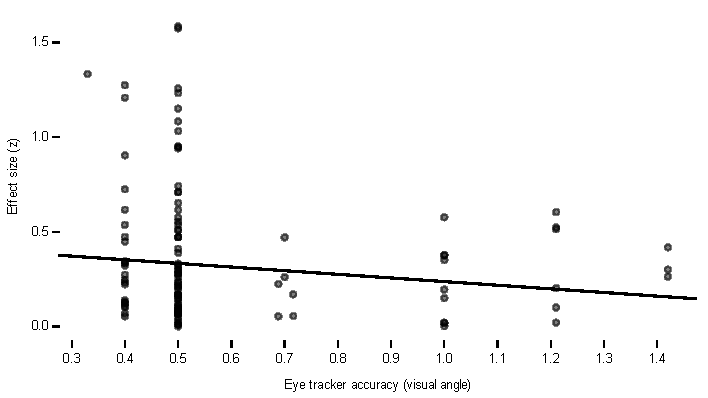
\includegraphics{ET_accuracy_effectsize}
\centering
\caption{Accuracy of the eye-tracker affects the ability to reliably measure effect sizes in each study. Points denote accuracy of an eye-tracker used in a study and absolute effect size (all converted to correlation coefficients) measured with it. The line is based on the estimated intercept and slope from the best fitting mixed-effect model which was used to compute artifact multiplier, $a_a$. The multiplier was used to correct for a bias in estimated effect sizes due to differences in measurement accuracy of eye-trackers.}
\label{fig:ET_accuracy_effectsize}
\end{figure}
\clearpage


% \caption{eye-tracker specifications table}
% \label{tab:eyetracker_specs}
% latex table generated in R 3.5.2 by xtable 1.8-4 package
% Mon Nov 30 09:54:56 2020
\begin{table}[ht]
\centering
\caption{Eye tracker specifications table, with accuracy and precision for each eye tracker as extracted from the manufacturer website, and computed artifact multiplier used for correcting for a bias in effect size estimates.} 
\label{tab:eyetracker_specifications}
\begin{tabular}{lccc}
  \hline
Eye tracker model & $a_a$ & Accuracy & Precision \\ 
  \hline
ASL6000 & 0.5523 & 1.00 & 0.50 \\ 
  Easygaze & 0.6866 & 0.70 & 0.35 \\ 
  Eye gaze 97 & 0.6794 & 0.72 & 0.50 \\ 
  Eye gaze tm & 0.8209 & 0.40 & 0.50 \\ 
  EyeLink 1000 & 0.7762 & 0.50 & 0.05 \\ 
  EyeLink 1000 (acc = .33) & 0.8523 & 0.33 & 0.05 \\ 
  EyeLink 1000 Plus (acc < .5) & 0.7762 & 0.50 & 0.05 \\ 
  EyeLink II & 0.7762 & 0.50 & 0.01 \\ 
  ISCAN & 0.5523 & 1.00 & 0.50 \\ 
  Nihon-Kohden EEG-1100 & 0.5523 & 1.00 & 0.50 \\ 
  SMI Glasses & 0.4583 & 1.21 & 0.19 \\ 
  SMI RED & 0.8209 & 0.40 & 0.03 \\ 
  SMI iview & 0.7762 & 0.50 & 0.01 \\ 
  SMI iview HED & 0.5523 & 1.00 & 0.50 \\ 
  SMI model unknown (acc < .5) & 0.7762 & 0.50 & 0.30 \\ 
  Tobii D10 & 0.7762 & 0.50 & 0.50 \\ 
  Tobii Glasses 1 & 0.3643 & 1.42 & 0.50 \\ 
  Tobii T120 & 0.8209 & 0.40 & 0.24 \\ 
  Tobii T1750 & 0.7762 & 0.50 & 0.25 \\ 
  Tobii T2150 & 0.7762 & 0.50 & 0.35 \\ 
  Tobii T60 & 0.7762 & 0.50 & 0.22 \\ 
  Tobii X1 & 0.7762 & 0.50 & 0.20 \\ 
  Tobii X2 & 0.8209 & 0.40 & 0.32 \\ 
  Tobii X60 & 0.7762 & 0.50 & 0.30 \\ 
  Tobii glasses 2 & 0.3643 & 1.42 & 0.34 \\ 
  Unknown & 0.6919 & 0.69 & 0.30 \\ 
   \hline 
 \multicolumn{4}{l}{\scriptsize{\textit{Note.} $a_a$ = artifact multiplier.}} 
\end{tabular}
\end{table}

\clearpage


\begin{figure}%[H]
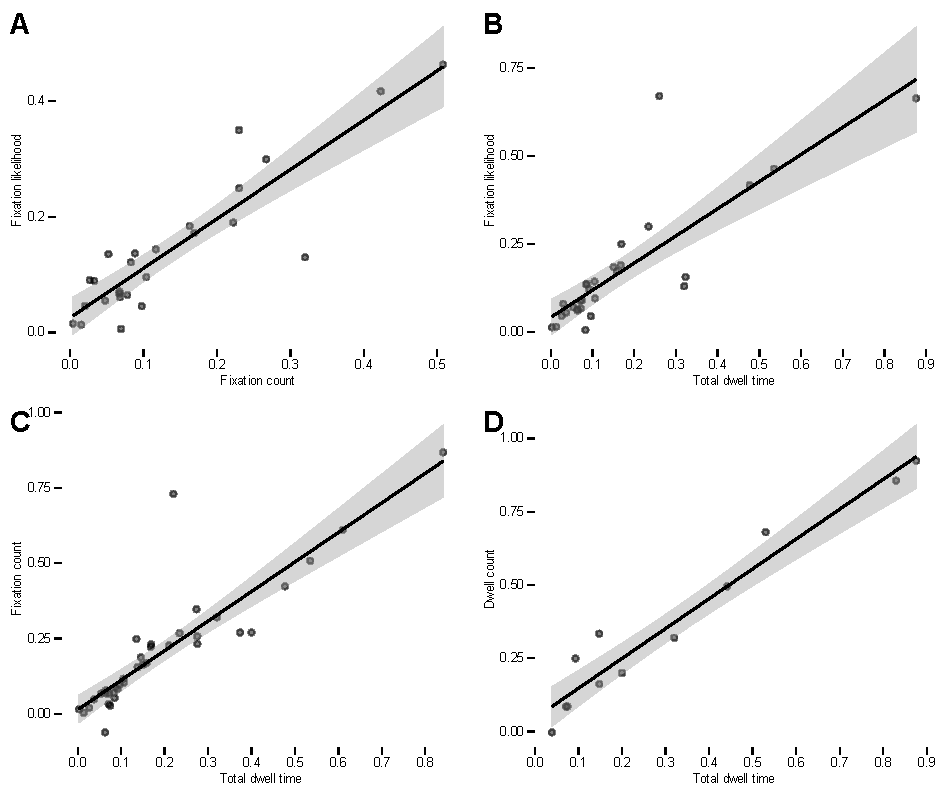
\includegraphics{metric_correction}
\centering
\caption{A variety of eye movement measures are used as a metric for dependent variable, but they are all highly correlated, suggesting they are all measuring the same underlying construct. Scatterplots show the relationship (A) between effect sizes expressed in fixation likelihood and fixation count, (B) between total fixation duration and fixation likelihood, (C) between total fixation duration and fixation count, (D) between total fixation duration and dwell count. Lines in each plot represent the best-fitting linear regression line, and the shaded area 95\% confidence interval.}
\label{fig:metric_correction}
\end{figure}
\clearpage


% \caption{Metric correction factor $a_m$ when correcting to either fixation count or fixation likelihood}
% \label{tab:metric_correction}
% latex table generated in R 3.6.3 by xtable 1.8-4 package
% Fri Dec 18 00:07:07 2020
\begin{table}[ht]
\centering
\caption{Metric correction factor $a_m$ when correcting to either fixation count or fixation likelihood. These correction factors were used to make sure all dependent variables are comparable.} 
\label{tab:metric_correction}
\begin{tabular}{llc}
  \hline
Correcting from & Correcting to & $a_m$ \\ 
  \hline
Fixation count & Fixation likelihood & 1.041 \\ 
  Fixation likelihood & Fixation count & 0.961 \\ 
  Total dwell time & Fixation likelihood & 0.913 \\ 
  Total dwell time & Fixation count & 1.035 \\ 
  Dwell count & Fixation likelihood & 0.844 \\ 
  Dwell count & Fixation count & 0.957 \\ 
   \hline
\end{tabular}
\end{table}

\clearpage


% \caption{Moderator analysis results.}
% \label{tab:mod_results}
% latex table generated in R 3.5.2 by xtable 1.8-4 package
% Mon Apr 19 09:34:50 2021
\begin{table}[ht]
\centering
\caption{Moderator analysis results. The most important values are the corrected effect size estimate, $\rho$, and the associated heterogeneity, $I^2$. 
                Results of the Top10 analysis are in parentheses.} 
\label{tab:mod_results}
\begingroup\small
\begin{tabular}{lccccccccc}
  \hline
Group & $k$ & $N$ & $\rho$ & SE & $Z$ & $p$ & $\textrm{CI}^{95}_{LL}$ & $\textrm{CI}^{95}_{UL}$ & $I^2$ \\ 
  \hline
\textbf{Set size} &  &  &  &  &  &  &  &  &  \\ 
  \hspace{2mm}\textit{Alternative} & 6 & 281 & 0.5 & 0.01 & 48.55 & <0.001 & 0.45 & 0.54 & 0 \\ 
   & (2) & (146) & (0.52) & (0.09) & (6.01) & (<0.001) & (0.35) & (0.69) & (0) \\ 
  \hspace{2mm}\textit{Attribute} & 7 & 726 & 0.14 & 0.05 & 2.88 & 0.035 & 0.02 & 0.27 & 30.38 \\ 
   & (2) & (302) & (0.07) & (0.07) & (0.95) & (0.343) & (-0.07) & (0.21) & (0) \\ 
  \textbf{Task instruction} &  &  &  &  &  &  &  &  &  \\ 
  \hspace{2mm}\textit{Alternative} & 12 & 787 & 0.39 & 0.08 & 4.79 & 0.001 & 0.2 & 0.57 & 10.85 \\ 
   & (2) & (406) & (0.34) & (0.11) & (3.13) & (0.002) & (0.13) & (0.56) & (38.13) \\ 
  \hspace{2mm}\textit{Attribute} & 16 & 1273 & 0.34 & 0.06 & 5.32 & <0.001 & 0.2 & 0.48 & 64.64 \\ 
   & (2) & (468) & (0.28) & (0.1) & (2.67) & (0.008) & (0.07) & (0.48) & (68.33) \\ 
  \textbf{Preferential viewing} &  &  &  &  &  &  &  &  &  \\ 
  \hspace{2mm}\textit{Alternative} & 7 & 600 & 0.61 & 0.19 & 3.17 & 0.034 & 0.08 & 1.13 & 76.81 \\ 
   & (2) & (385) & (0.29) & (0.08) & (3.64) & (<0.001) & (0.13) & (0.45) & (0) \\ 
  \hspace{2mm}\textit{Attribute} & 17 & 2033 & 0.31 & 0.08 & 3.95 & 0.002 & 0.14 & 0.47 & 77.03 \\ 
   & (2) & (688) & (0.31) & (0.13) & (2.43) & (0.015) & (0.06) & (0.55) & (86.6) \\ 
   \hline 
 \multicolumn{10}{p{0.9\textwidth}}{\scriptsize{\textit{Note.} $k$ = number of studies; $N$ = number of participants; $\rho$ = unattenuated effect size estimate, SE = standard error of estimate; $Z$ = Z statistic; $p$ = significance level; $\textrm{CI}^{95}_{LL}$ = lower limit of the 95\% confidence interval; $\textrm{CI}^{95}_{LL}$ = upper limit of the 95\% confidence interval, $I^2$ = within-group heterogeneity.}} 
\end{tabular}
\endgroup
\end{table}

\clearpage


\begin{figure}%[H]
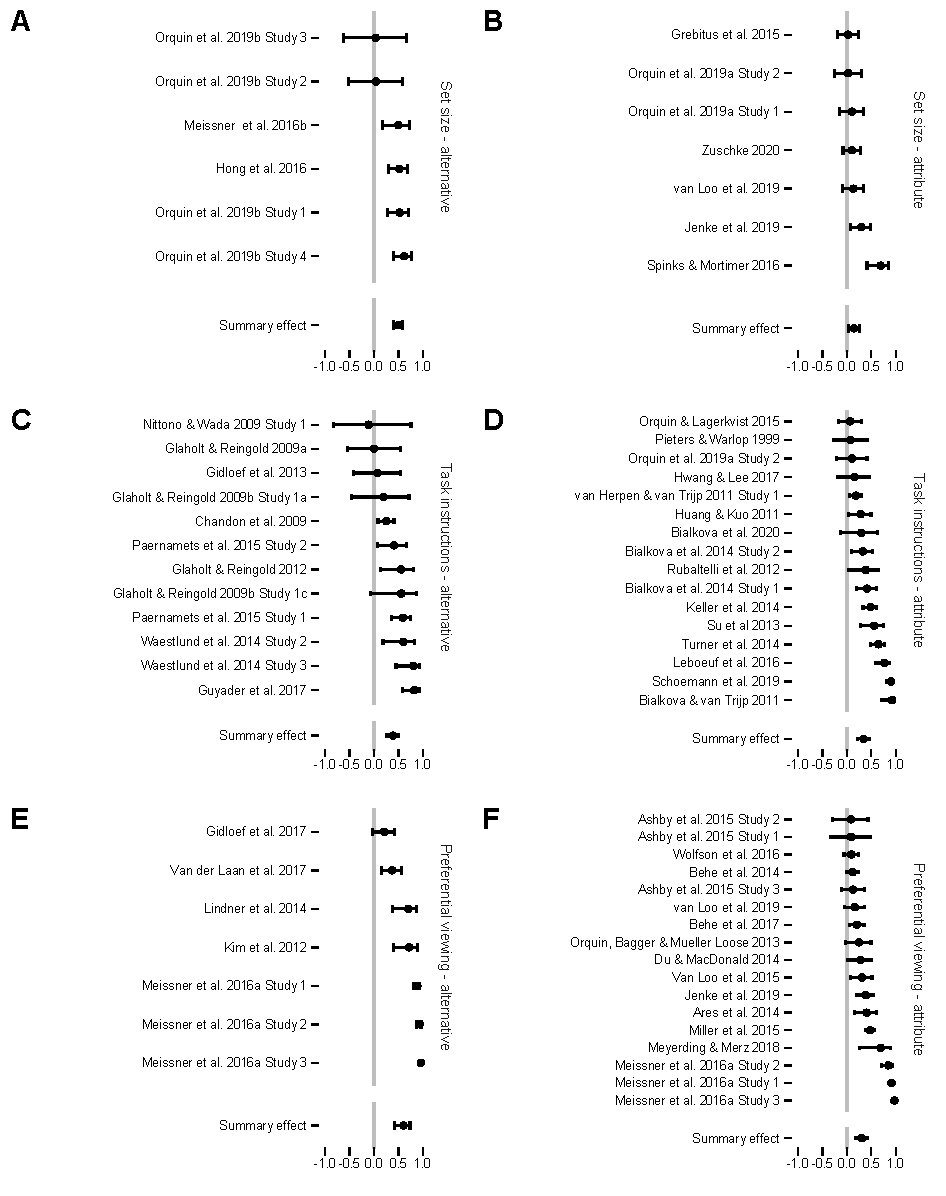
\includegraphics{forest_plots_altatt}
\centering
\singlespace
\caption{Effect sizes of the factors that were decomposed into alternative and attribute parts for moderator analyses. Forest plots show the unattenuated effect size correlations for each study in a group, as well as average effect across the group. Forest plot in (A) shows the effect sizes for set size -- alternative, in (B) for set size -- attribute, in (C) for task instructions -- alternative, in (D) for task instructions -- attribute, in (E) for preferential viewing -- alternative, and in (F) for preferential viewing -- attribute. Error bars represent the 95\% confidence interval around the mean.}
\label{fig:forest_plots_altatt}
\end{figure}
\clearpage


\begin{figure}%[H]
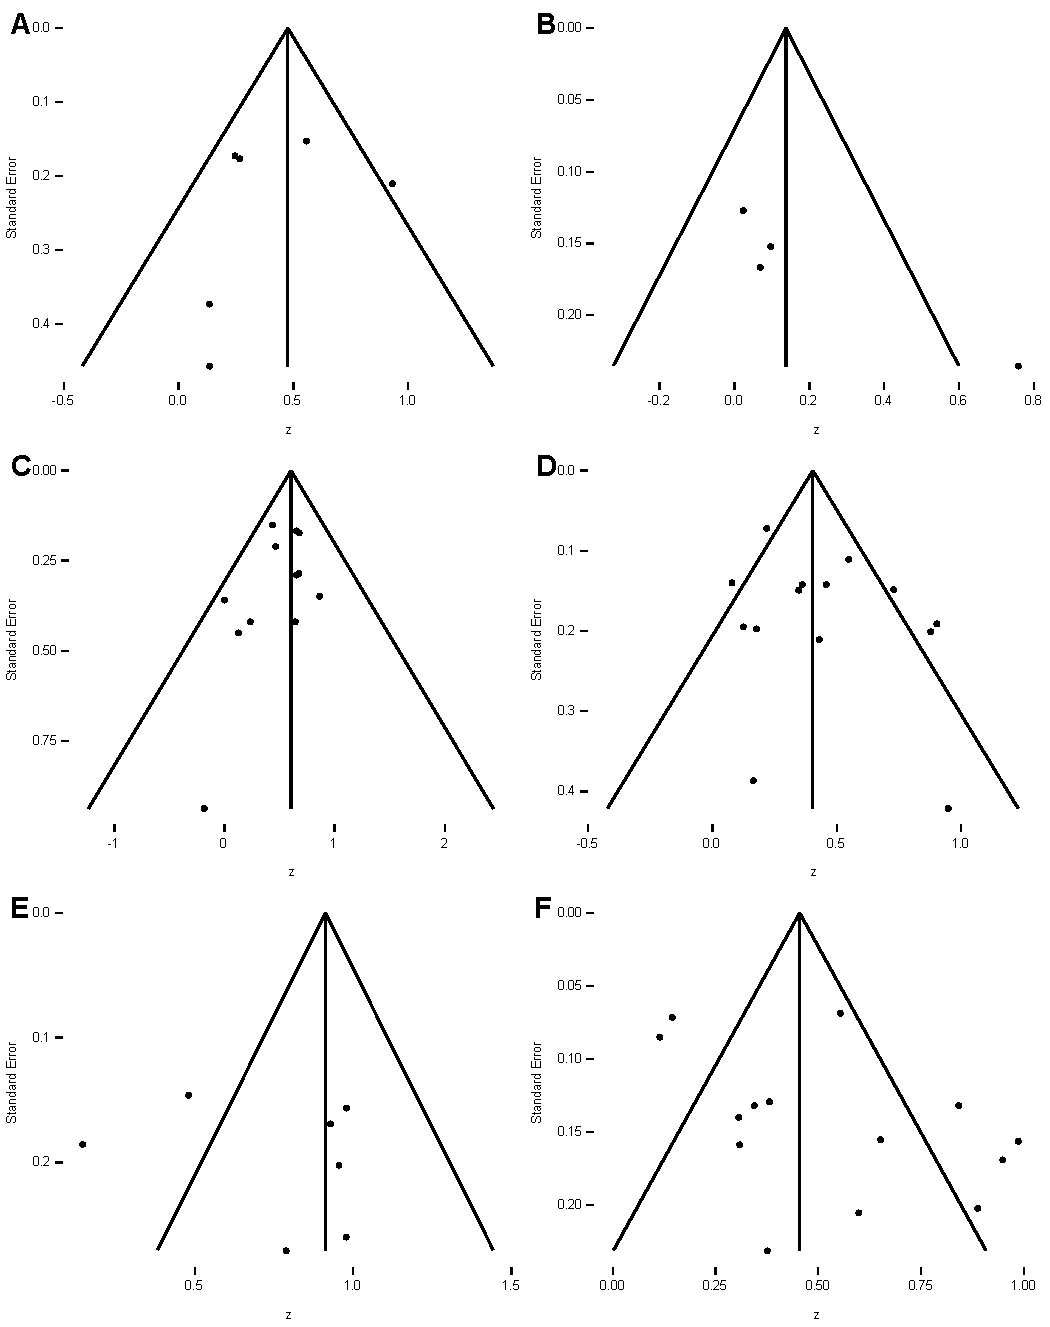
\includegraphics{funnel_plots_altatt}
\centering
\singlespace
\caption{Funnel plots for factors that were decomposed into alternative and attribute parts for moderator analyses. Points are Fisher transformed correlation coefficients against their standard error. Asymmetric distributions of points can indicate the presence of publication bias since smaller studies (those with higher standard errors) have more variable effect sizes and are less likely to be published unless the effect is large. Funnel plot for (A) set size -- alternative, (B) set size -- attribute, (C) task instructions -- alternative, (D) task instructions -- attribute, (E) preferential viewing -- alternative, (F) preferential viewing -- attribute.}
\label{fig:funnel_plots_altatt}
\end{figure}
\clearpage

\end{document}